\chapter{\texorpdfstring{\(SU(5)\)}{SU(5)}の多重項、レプトクォークゲージボソン、陽子崩壊}

\lectureoverview{標準模型の群が\(SU(5)\)に埋め込まれると、大統一は具体的なものになる。その意味を理解するために、まず必要な表現論を構築する。定義表現\(N\)、その共役\(\overline N\)、テンソル積、対称テンソルと反対称テンソル、そして随伴表現である。すると標準模型の1世代は、予想外に経済的な組み合わせ\(\overline{\mathbf 5}\oplus\mathbf{10}\)に収まる。この配置を美しくしているのと同じ対称性が、クォークをレプトンに変換するカラーゲージボソンを要求する。それらの交換は陽子崩壊を許し、統一スケールを\(10^{15}\)--\(10^{16}\,\mathrm{GeV}\)へと押しやる。走るゲージ結合定数は同程度のスケールを指し示し、最後に超対称性が再び現れる。それはそれらの数値的な一致を大幅に鋭くするからである。}

\section{なぜ群の表現から始めるのか？}

提案されている大統一理論は数多くある。それらを概観するのではなく、1つの例を取り上げて3つの問いを立てる。何がそれを機能させるのか、どのような新しい粒子を必要とするのか、そして実験はどこでそれを危険にさらすのか。群は\(SU(5)\)であり、その定義的な構造的特徴は埋め込み
\begin{equation}
SU(3)_c\times SU(2)_L\times U(1)_Y
\subset SU(5).
\label{eq:l10-sm-embedding}
\end{equation}
である。ここで\(SU(3)_c\)はカラーに、\(SU(2)_L\)は弱アイソスピンに、\(U(1)_Y\)はハイパーチャージに作用する。

超対称性はこの構成の前提ではない。超対称性も大統一も、論理的に他方を含意しない。この講義における両者の結びつきは数値的である。超対称パートナーのスペクトルを繰り込み群の計算に含めると、3つのゲージ結合定数はより正確に共通の値に近づく。

対称性が互いに混合する粒子は、その対称性群の表現を形成する。したがって、統一された粒子多重項を分類するには、まず少しの表現論が必要である。

\subsection{おなじみの\texorpdfstring{\(SU(2)\)}{SU(2)}の例}

通常の角運動量に対応する\(SU(2)\)は、三次元空間の回転と密接に関係している。より正確には、\(SU(2)\)は\(SO(3)\)の二重被覆である。その既約表現は
\begin{equation}
j=0,\frac12,1,\frac32,\ldots,
\qquad
\dim(j)=2j+1.
\label{eq:l10-su2-spins}
\end{equation}
によってラベル付けられる。したがって、スカラーは一重項であり、スピン\(\tfrac12\)の粒子は二重項であり、スピン1の粒子は三重項である。弱い群\(SU(2)_L\)は、その抽象的な群論は同じであるが、異なる物理的対称性である。

\section{定義表現とその共役}

\(SU(N)\)に対して、定義表現は複素\(N\)成分の列の空間であり、
\begin{equation}
\psi=
\begin{pmatrix}
\psi_1\\
\psi_2\\
\vdots\\
\psi_N
\end{pmatrix},
\qquad
\psi'_i=U_i{}^j\psi_j,
\qquad
U\in SU(N).
\label{eq:l10-defining}
\end{equation}
である。これは定義表現、または単に\(\mathbf N\)と呼ばれる。行列\(U\)は\(N\times N\)であり、それらが作用するベクトル空間の次元は\(N\)である。

複素共役は別の\(N\)次元表現を与え、
\begin{equation}
\psi_i^*\longmapsto U_i{}^{j*}\psi_j^*,
\label{eq:l10-conjugate}
\end{equation}
と表され、\(\overline{\mathbf N}\)と記される。\(N>2\)に対して、定義表現と共役表現は同値でない。どちらを粒子表現と呼び、どちらを反粒子表現と呼ぶかは交換できるが、一度規約を選んだらそれを固定しておかなければならない。

\begin{classroomqa}
\audiencequestion{\(SU(N)\)における\(N\)は、\(N\)が偶数か奇数かに依存するのか、またそれは行列を指すのか？\lecturetimestamp{00:07:33}}
\lecturerresponse{ここには偶数--奇数という制限はない。\(N\)は定義行列の大きさであり、同時にそれらの定義表現の次元でもある。\(\mathbf N\)も\(\overline{\mathbf N}\)もその次元を持つ。}
\end{classroomqa}

反粒子の反粒子は元の粒子である。これが、\(\mathbf N\)と\(\overline{\mathbf N}\)の名前を交換することが物理ではなく規約を変える理由である。

\section{テンソル積と既約性}

一方の物体が\(N\)個の内部状態を占めることができ、もう一方の物体が独立に同じ数を占めることができるとする。位置、運動量、スピン、およびこの\(SU(N)\)ラベル以外のすべての量子数を無視すると、その対は
\begin{equation}
N\times N=N^2
\label{eq:l10-product-count}
\end{equation}
個の状態を持つ。第1の物体が状態\(\psi_i\)にあり、第2の物体が状態\(\phi_j\)にあるなら、それらの積は
\begin{equation}
\Psi_{ij}=\psi_i\phi_j,
\qquad
\Psi'_{ij}=U_i{}^kU_j{}^\ell\Psi_{k\ell}.
\label{eq:l10-tensor-transform}
\end{equation}
と書ける。これがテンソル積\(\mathbf N\otimes\mathbf N\)である。

\begin{classroomqa}
\audiencequestion{なぜ答えは\(N^2-1\)ではなく\(N^2\)なのか、また両方の粒子に同じ内部ラベルを許すことは排他原理に違反しないのか？\lecturetimestamp{00:10:22}}
\lecturerresponse{ここでは2つのスロットは区別可能である。一方の物体はある位置に固定され、他方は別の位置にある。パウリ原理は位置を含む完全な量子状態を制約する。それはこれらの\(N^2\)個の内部ラベルの組み合わせのいずれも排除しない。数\(N^2-1\)は後に、別の積におけるトレースレス条件から現れる。}
\end{classroomqa}

\(N^2\)次元の積表現は一般に可約である。表現が可約であるとは、群がそれ自身へ写す真部分空間を含む場合をいう。不変部分空間は分離してより小さな表現として扱うことができ、そのような真部分空間が存在しなければ、その表現は既約である。

\subsection{対称テンソルと反対称テンソル}

2添字テンソルはすべて一意的に
\begin{align}
\Psi_{ij}
&=\Psi^{(S)}_{ij}+\Psi^{(A)}_{ij},\\
\Psi^{(S)}_{ij}
&=\frac12(\Psi_{ij}+\Psi_{ji}),\\
\Psi^{(A)}_{ij}
&=\frac12(\Psi_{ij}-\Psi_{ji}).
\label{eq:l10-sym-anti}
\end{align}
と分解される。2つの部分は
\begin{equation}
\Psi^{(S)}_{ij}=\Psi^{(S)}_{ji},
\qquad
\Psi^{(A)}_{ij}=-\Psi^{(A)}_{ji}.
\end{equation}
を満たす。式~\eqref{eq:l10-tensor-transform}はそれぞれの条件を保つので、群変換が対称部門と反対称部門を混ぜることは決してない。

\editorialnote{講義では一般的な数え上げを演習として残している。対称次元と反対称次元はそれぞれ\(N(N+1)/2\)および\(N(N-1)/2\)であり、それらの和は\(N^2\)である。}

\begin{figure}[htbp]
\centering
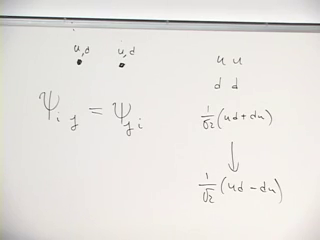
\includegraphics[width=0.78\textwidth]{lecture_10_figure_02.png}
\lectureframe{00:17:57.500}
\caption{スピン\(\tfrac12\)状態2つの完成した板書の分解：3つの対称状態と1つの反対称状態。}
\label{fig:l10-spin-decomposition}
\end{figure}

\(SU(2)\)の定義二重項に対して、
\begin{equation}
\mathbf2\otimes\mathbf2=\mathbf3_S\oplus\mathbf1_A.
\label{eq:l10-two-two}
\end{equation}
2つの基底状態を\(u\)および\(d\)と書くと、対称三重項は
\begin{align}
\ket{1,1}&=\ket{uu},\\
\ket{1,0}&=\frac{1}{\sqrt2}\bigl(\ket{ud}+\ket{du}\bigr),\\
\ket{1,-1}&=\ket{dd},
\end{align}
であり、反対称一重項は
\begin{equation}
\ket{0,0}
=\frac{1}{\sqrt2}\bigl(\ket{ud}-\ket{du}\bigr).
\end{equation}
である。これは2つのスピン\(\tfrac12\)角運動量のよく知られた合成である。4つの生の状態はスピン1とスピン0に再編成される。

\section{粒子と反粒子：随伴表現}

次に定義表現とその共役を組み合わせる。積は依然として\(N^2\)個の成分をもつが、行列として変換する：
\begin{equation}
M_i{}^j\in\mathbf N\otimes\overline{\mathbf N},
\qquad
M\longmapsto U M U^\dagger.
\label{eq:l10-matrix-transform}
\end{equation}
\(\mathbf N\otimes\mathbf N\)とは異なり、1つの基本添字と1つの反基本添字の間には意味のある交換対称性はない。自然な分解は代わりに
\begin{equation}
M
=
\frac{\operatorname{tr}M}{N}\,\mathbf1_N
+
\left(M-\frac{\operatorname{tr}M}{N}\,\mathbf1_N\right).
\label{eq:l10-trace-split}
\end{equation}
である。第1項は一重項であり、トレースレス部分は随伴表現である：
\begin{equation}
\mathbf N\otimes\overline{\mathbf N}
=\mathbf1\oplus\mathbf{Adj},
\qquad
\dim\mathbf{Adj}=N^2-1.
\label{eq:l10-adjoint}
\end{equation}

\begin{figure}[htbp]
\centering
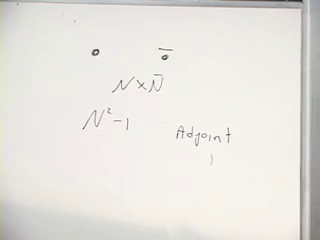
\includegraphics[width=0.67\textwidth]{lecture_10_figure_04.png}
\lectureframe{00:23:47.500}
\caption{\(\mathbf N\otimes\overline{\mathbf N}\)についての板書の結論：そのトレースレスな\(N^2-1\)個の成分が随伴表現をなす。}
\label{fig:l10-adjoint}
\end{figure}

\(SU(3)\)に対して、これはよく知られた八重項を与え、
\begin{equation}
\mathbf3\otimes\overline{\mathbf3}
=\mathbf8\oplus\mathbf1,
\end{equation}
8つのグルーオンは随伴表現で変換する。\(SU(2)\)に対して、随伴表現は次元3をもち、スピン1のように変換する。

\section{標準模型の1世代}

観測されている世代は3つあるが、\(SU(5)\)は同じ構成を各世代について別々に繰り返す。なぜ3つのコピーが存在するのかは説明しない。したがって我々は第1世代に焦点を当てる。

場はすべて左手ワイル場として書かれる。右手フェルミオンはその左手電荷共役場によって表される：
\begin{equation}
u^c_L,\qquad d^c_L,\qquad e^c_L.
\label{eq:l10-left-handed-bookkeeping}
\end{equation}
上付き添字\(c\)は電荷共役を表す。たとえば\(d^c_L\)は電荷\(+\tfrac13\)をもつ左手反ダウン場である。

標準的な\(SU(5)\)記法では、15個の左手場のうち5個が
\begin{equation}
\overline{\mathbf5}
=
\begin{pmatrix}
\nu_{eL}\\
e_L\\
d^c_{rL}\\
d^c_{gL}\\
d^c_{bL}
\end{pmatrix}.
\label{eq:l10-fivebar}
\end{equation}
に収まる。順序は弱2次元ブロックの後に色3次元ブロックが続くように選ばれている。弱変換は最初の2つの成分を混ぜ、色変換は最後の3つを混ぜ、非対角な\(SU(5)\)生成子は2つのブロックを結ぶ。

\editorialnote{講義では式~\eqref{eq:l10-fivebar}の列を\(\mathbf5\)と呼び、後に反対称多重項を\(\overline{\mathbf{10}}\)と呼んでいる。これは大域的に共役な規約である。我々は現代の標準的な\(\overline{\mathbf5}\oplus\mathbf{10}\)を用いる。すべての表現を共役にすれば、物理学を変えることなく講義のラベルが再現される。}

最小の第1世代の完全な目録は
\begin{equation}
\begin{gathered}
\underbrace{Q_L=(u_L,d_L)}_{6}
\oplus
\underbrace{L_L=(\nu_{eL},e_L)}_{2},\\
\underbrace{u^c_L}_{3}
\oplus
\underbrace{d^c_L}_{3}
\oplus
\underbrace{e^c_L}_{1},\\
6+2+3+3+1=15.
\end{gathered}
\label{eq:l10-fifteen}
\end{equation}
である。最小標準模型には独立な\(\nu^c_L\)がないので、繰り込み可能なニュートリノ質量を与えない。ニュートリノ振動はこの最小の主張が不完全であることを示している。すなわち自然は小さな非零のニュートリノ質量をもち、拡張が必要である。

\begin{classroomqa}
\audiencequestion{フェルミオン質量が左手状態を右手状態に変えるとき、それは粒子をその反粒子にも変えるのか。\lecturetimestamp{00:34:00}}
\lecturerresponse{いいえ。電子質量は左手電子を同じ電荷をもつ右手電子に結びつける。すべて左手の記法では第2の場は\(e^c_L\)で表されるが、4成分の粒子は依然として電子である。粒子と反粒子を同一視するマヨラナ質量をもちうるのは中性場だけである。}
\end{classroomqa}

\section{5重項に見えるゲージボソン}

ゲージ対称性の各生成子には対応するゲージ場がある。式~\eqref{eq:l10-fivebar}の中では、よく知られた遷移がすでに認識できる：
\begin{itemize}
\item 弱ゲージ場は\(\nu_{eL}\)と\(e_L\)の間で作用する。
\item グルーオンは\(d^c_L\)の3つの色の間で作用する。
\item 中性生成子は対角的に作用する。
\item 新しい非対角生成子はレプトン成分を色成分に、またはその逆に変換する。
\end{itemize}

グルーオンはクォーク--反クォークのカラー量子数を持つものとして描くことができる。講義では通常の世界線の記憶法を用いる。すなわち、出ていく反クォークを放出頂点を通って逆向きにたどると、前向きに走るクォークのように見える。したがって、放出される場はクォーク--反クォーク対の量子数を持つ。表現の言葉では、これはまさに\(\mathbf3\otimes\overline{\mathbf3}\)のトレースレス部分である。

\(SU(5)\)に対して、
\begin{equation}
\dim\mathbf{Adj}_{SU(5)}=5^2-1=24.
\end{equation}
これらのゲージ場の標準模型部分群の下での分解は
\begin{equation}
\mathbf{24}
=
(\mathbf8,\mathbf1)_0
\oplus(\mathbf1,\mathbf3)_0
\oplus(\mathbf1,\mathbf1)_0
\oplus(\mathbf3,\mathbf2)_{-5/6}
\oplus(\overline{\mathbf3},\mathbf2)_{5/6},
\label{eq:l10-adjoint-sm}
\end{equation}
である。ここで順序対は\(SU(3)_c\times SU(2)_L\)を表し、添字はハイパーチャージである。

\editorialnote{式~\eqref{eq:l10-adjoint-sm}は、講義で描かれたブロック構造を明示している。最初の3つの項は、おなじみのカラーおよび電弱ゲージ場を含む。最後の2つの項は、慣習的に\(X\)および\(Y\)ボソンと呼ばれる12個の実自由度である。}

\begin{figure}[htbp]
\centering
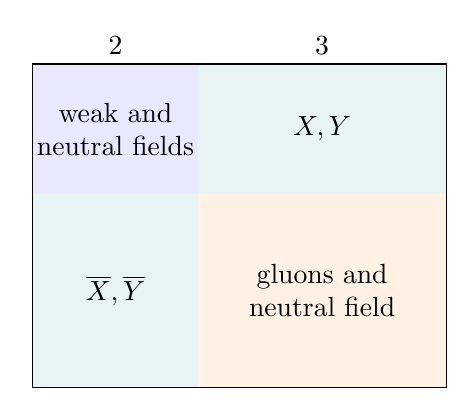
\begin{tikzpicture}[x=1.05cm,y=0.82cm]
  \draw[thick] (0,0) rectangle (5,5);
  \draw[thick] (2,0) -- (2,5);
  \draw[thick] (0,3) -- (5,3);
  \fill[blue!9] (0,3) rectangle (2,5);
  \fill[orange!10] (2,0) rectangle (5,3);
  \fill[teal!9] (2,3) rectangle (5,5);
  \fill[teal!9] (0,0) rectangle (2,3);
  \node[align=center] at (1,4) {weak and\\neutral fields};
  \node[align=center] at (3.5,1.5) {gluons and\\neutral field};
  \node[align=center] at (3.5,4) {\(X,Y\)};
  \node[align=center] at (1,1.5) {\(\overline X,\overline Y\)};
  \node[above] at (1,5) {\(2\)};
  \node[above] at (3.5,5) {\(3\)};
\end{tikzpicture}
\caption{\(SU(5)\)ゲージ場の\(2\oplus3\)ブロック構造。非対角ブロックはレプトンとカラー場を結ぶ。}
\label{fig:l10-gauge-blocks}
\end{figure}

\(Q=T_3+Y\)のもとで、式~\eqref{eq:l10-adjoint-sm}のカラー弱二重項は電荷\(-\tfrac13\)および\(-\tfrac43\)を持ち、その共役は\(+\tfrac13\)および\(+\tfrac43\)を持つ。講義ではこれらの粒子を\(X\)および\(Y\)と呼ぶが、どちらの名前がどちらの電荷に対応するかは明示的に定めない。遷移と電荷が不変な内容である。

\begin{classroomqa}
\audiencequestion{それぞれの新しい\(X\)または\(Y\)ゲージボソンには3つの版があるのか。\lecturetimestamp{00:41:28}}
\lecturerresponse{はい。遷移はカラーを持つクォークの成分をカラーを持たないレプトンの成分に結びつけるので、交換されるボソンは欠けているカラーを運ばなければならない。\(X/Y\)場はカラー三重項を形成し、グルーオンを放出または吸収することができる。}
\end{classroomqa}

カラーを持つ粒子は孤立した漸近状態として観測されない。新しいゲージボソンは、クォークと同様に、崩壊するかハドロン化してカラー中性の組み合わせにならなければならない。

\section{なぜ多重項が反ダウンクォークを含むのか}

\(SU(N)\)の生成子はトレースレスなエルミート行列である。specialという言葉との関係を見るために、無限小群要素を
\begin{equation}
U(\epsilon)=e^{i\epsilon T}.
\end{equation}
と書く。ユニタリ性から\(T^\dagger=T\)が得られ、一方、任意の\(\epsilon\)に対して
\begin{equation}
1=\det U=e^{i\epsilon\operatorname{tr}T}
\end{equation}
から
\begin{equation}
\operatorname{tr}T=0.
\label{eq:l10-traceless-generator}
\end{equation}
が得られる。

電荷は生成子の線形結合である。式~\eqref{eq:l10-fivebar}の物質列に対して、それは
\begin{equation}
Q_{\overline5}
=
\operatorname{diag}
\left(0,-1,\frac13,\frac13,\frac13\right),
\qquad
\operatorname{tr}Q_{\overline5}=0.
\label{eq:l10-charge-fivebar}
\end{equation}
として作用する。したがって
\begin{equation}
0-1+3\left(\frac13\right)=0.
\end{equation}
である。反ダウン場をダウン場に置き換えると代わりに
\begin{equation}
0-1+3\left(-\frac13\right)=-2,
\end{equation}
が得られるが、これは\(SU(5)\)生成子のトレースにはなり得ない。したがって、一見奇妙な反ダウンの割り当ては群構造によって強制される。

\section{残りの10個のフェルミオン}

他の10個の場は反対称な2添字テンソルから生じる。標準的な慣習では、これは
\begin{equation}
\mathbf5\otimes\mathbf5
=\mathbf{15}_S\oplus\mathbf{10}_A.
\label{eq:l10-five-five}
\end{equation}
の反対称部分である。講義では、一時的に共役量子数
\begin{equation}
\chi=
\begin{pmatrix}
\nu^c\\
e^c\\
d_r\\
d_g\\
d_b
\end{pmatrix}.
\label{eq:l10-aux-five}
\end{equation}
を書くことによってこれを構成する。これは表現をテンソル積にするための簿記上の工夫であり、複合粒子の第2の物理的な5重項が存在するという主張ではない。


\begin{equation}
\Psi^{ij}=-\Psi^{ji},
\qquad
i,j=1,\ldots,5.
\label{eq:l10-antisym-ten}
\end{equation}
とする。すべての対角成分は消え、下三角は上三角によって固定される。したがって
\begin{equation}
\dim\mathbf{10}
=\binom52
=\frac{5\cdot4}{2}
=10.
\label{eq:l10-ten-count}
\end{equation}
である。

成分の電荷は、式~\eqref{eq:l10-aux-five}の行と列の電荷の和である。これにより直ちに、弱--弱スロットに\(e^c\)、弱--カラーブロックにダウンクォークとアップクォーク、カラー--カラーブロックに反アップ場が得られる。

\begin{classroomqa}
\audiencequestion{陽電子とダウンクォークのラベルを組み合わせると、結果の成分は\(X\)ボソンになるべきか。\lecturetimestamp{00:53:08}}
\lecturerresponse{いいえ。この段階ではフェルミオン表現を構成しており、ゲージボソンの随伴表現ではない。電荷は\(1-\tfrac13=\tfrac23\)として加わるので、その成分はアップクォークの量子数を持つ。}
\end{classroomqa}

カラーの符号の整合的な選択は
\begin{equation}
\Psi^{ij}=
\begin{pmatrix}
0 & e^c & d_r & d_g & d_b\\
-e^c & 0 & u_r & u_g & u_b\\
-d_r & -u_r & 0 & u_b^c & -u_g^c\\
-d_g & -u_g & -u_b^c & 0 & u_r^c\\
-d_b & -u_b & u_g^c & -u_r^c & 0
\end{pmatrix}.
\label{eq:l10-ten-matrix}
\end{equation}
である。場の位相を変えると表示される符号のいくつかは変わるが、表現や粒子内容は変わらない。

\begin{figure}[htbp]
\centering
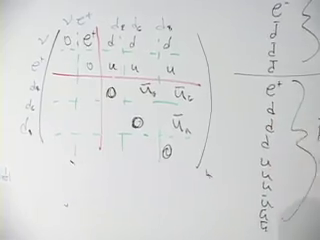
\includegraphics[width=0.83\textwidth]{lecture_10_figure_05.png}
\lectureframe{00:59:17.500}
\caption{授業で成分とカラーラベルを確認した後の、妨げのない\(2\oplus3\)反対称物質行列。}
\label{fig:l10-ten-board}
\end{figure}

\begin{classroomqa}
\audiencequestion{10次元表現は行列として書かなければならないのか、それとも列として書くことができるのか。\lecturetimestamp{00:56:24}}
\lecturerresponse{どちらも可能である。10個の独立成分を列に並べることもできるが、反対称な\(5\times5\)行列は\(SU(5)\)がその2つの添字にどのように作用するかを示すので、はるかに情報量が多い。}
\end{classroomqa}

\begin{classroomqa}
\audiencequestion{カラー--カラーブロックにおいて、\(u\)と記された項目は実際には反アップ場であるべきか？ \lecturetimestamp{00:57:51}}
\lecturerresponse{はい。ボードのラベルは\(u^c\)、すなわち左手系の反アップ場に訂正される。2つのダウン型基底電荷の和は\(-\tfrac23\)となり、これは反アップクォークの電荷である。}
\end{classroomqa}

\begin{classroomqa}
\audiencequestion{いくつかの行列要素からカラーが省略されている。それらは依然として保存されているのか？ \lecturetimestamp{00:58:05}}
\lecturerresponse{はい。3つのカラースロットは赤、緑、青である。ラベルは煩雑さを減らすためにのみ省略された。}
\end{classroomqa}

カラー基本表現の反対称な対は反カラーとして変換する：
\begin{equation}
\wedge^2\mathbf3\simeq\overline{\mathbf3},
\qquad
(rg,rb,gb)\sim(\overline b,-\overline g,\overline r).
\label{eq:l10-anticolor}
\end{equation}
これが、カラー--カラーブロックにおける3つの独立な項目がまさに反アップカラー三重項を形成する理由である。

1世代は今や次のように整理された：
\begin{equation}
\overline{\mathbf5}\oplus\mathbf{10}.
\label{eq:l10-family}
\end{equation}
\(u_L\)と\(u^c_L\)が1つの既約多重項内に現れる一方、\(d_L\)と\(d^c_L\)、あるいは\(e_L\)と\(e^c_L\)は異なる多重項に属するのは注目に値する。

\begin{classroomqa}
\audiencequestion{ゲージ変換が各表現の内部でのみ作用するならば、質量はどのようにして5バーと10に属する場を結びつけることができるのか？ \lecturetimestamp{01:00:40}}
\lecturerresponse{ゲージボソンは1つの既約物質表現を他の表現へ回転させることはない。ヒッグス場と湯川結合は、全体として\(SU(5)\)不変な相互作用を形成しつつ異なる表現を結びつけることができ、ヒッグス場が期待値を獲得した後、それらの相互作用が質量を生成する。}
\end{classroomqa}

\section{ゲージボソンはシフトとして作用する}

表現が組み立てられた後、ゲージボソンの作用はその項目間のシフトとして読み取ることができる。中性ボソンはラベルを変えずに保つことができ、弱ゲージボソンは弱スロット間を移動し、グルーオンはカラースロット間を移動し、\(X/Y\)ボソンは弱スロットとカラースロットの間を移動する。荷電ゲージボソンには反粒子があるため、各シフトには逆過程が存在する。

反対称テンソルに対して、無限小変換はどちらかの添字に作用する：
\begin{equation}
\delta\Psi^{ij}
=
i\epsilon
\left(
T^i{}_k\Psi^{kj}
+
T^j{}_k\Psi^{ik}
\right).
\label{eq:l10-two-index-action}
\end{equation}
行列の描像では、第1項は縦に動き、第2項は横に動く。テンソルを構成するために用いられた構成ラベルは単なる記憶補助にすぎず、式~\eqref{eq:l10-two-index-action}が正確な群論的記述である。

弱シフトは\(d\)を\(u\)へと移す。これは中性子ベータ崩壊の背後にあるクォークレベルの過程である。カラーシフトはフレーバーを変えずに赤、緑、青を変化させる。非対角シフトは新しいことを行う：
\begin{equation}
\begin{aligned}
d^c&\longleftrightarrow e,
& d^c&\longleftrightarrow\nu,\\
d&\longleftrightarrow u^c,
& u&\longleftrightarrow e^c,
\end{aligned}
\label{eq:l10-leptoquark-shifts}
\end{equation}
ここで適切な\(X/Y\)場が電荷とカラーの差を担う。

\begin{classroomqa}
\audiencequestion{第四スロットと第五スロットの間の移行は何を表すのか、また第一スロットから第四スロットへの移行はどうか。\lecturetimestamp{01:10:36}}
\lecturerresponse{第四--第五の移行は一つの色を別の色に変え、グルーオン遷移である。第一--第四の移行は弱ブロックと色ブロックの間を横断し、新しい\(X/Y\)遷移の一つである。}
\end{classroomqa}

\begin{classroomqa}
\audiencequestion{反対称行列の下半分の1つの項目を明示的に埋めることができるか？ \lecturetimestamp{01:11:23}}
\lecturerresponse{はい。すべての下三角項目は転置された上三角項目の負である。1つを埋めれば規則が見えるようになり、すべてを埋めても新しい状態は加わらない。}
\end{classroomqa}

\section{危険な帰結：陽子崩壊}

\(X/Y\)ボソンは一方の頂点でクォークをレプトンに結合し、他方の頂点で2つのクォーク型場を結合することができる。その質量よりはるかに小さい運動量では、重いボソンを積分消去すると、概略的に次の形の6次元相互作用が得られる：
\begin{equation}
\mathcal L_{\mathrm{eff}}
\sim
\frac{g_5^2}{M_X^2}\,(qq)(q\ell)
+\text{h.c.}
\label{eq:l10-effective-proton}
\end{equation}
これはバリオン数とレプトン数を別々に破りながら、統一ゲージ相互作用によって課される組み合わせを保存する。

ボードは1つのダウンクォークと1つのアップクォークを重い交換を通して追跡する。ダウンクォークは陽電子になり、アップクォークは反アップクォークになり、第2のアップクォークは観測者である：
\begin{equation}
uud
\longrightarrow
e^++u\overline u.
\label{eq:l10-quark-decay}
\end{equation}
初期状態は陽子である。\(u\overline u\)対は中性パイオンへハドロン化することができ、次を与える：
\begin{equation}
p\longrightarrow e^++\pi^0.
\label{eq:l10-proton-pion}
\end{equation}

\begin{figure}[htbp]
\centering
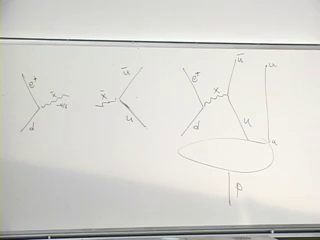
\includegraphics[width=0.82\textwidth]{lecture_10_figure_06.png}
\lectureframe{01:16:02.500}
\caption{陽子内部における重いボソン交換の完成されたボード構成。観測者アップクォークと陽電子チャネルが見える。}
\label{fig:l10-proton-board}
\end{figure}

講義では\(p\to e^++\gamma\)にも言及している。そこではクォーク--反クォーク対が電磁的に消滅する。そのチャネルは直接ハドロン化に対して追加の電磁的抑制を伴う。

この可能性はモデルの任意の装飾ではない。単純群がクォークとレプトンを結びつける生成子を含むならば、バリオン数を破る過程は一般に予想される。それらが通常の弱い相互作用や電磁相互作用の時間スケールで起こるならば、原子核、水素、巨視的物質は生き残れないであろう。

\section{なぜ陽子はそれほど長寿命なのか？}

\begin{classroomqa}
\audiencequestion{\(X\)ボソンを生成する結合は、群の残りの部分が用いるのと同じ大統一結合なのですか？\lecturetimestamp{01:18:34}}
\lecturerresponse{大統一スケールでは、はい。単純な\(SU(5)\)ゲージ理論は1つのゲージ結合\(g_5\)をもつ。低エネルギーの強い結合、弱い結合、ハイパーチャージ結合が異なるのは、大統一対称性が破れた後でそれらが異なる走り方をするからである。}
\end{classroomqa}

統一構造を放棄することなく、結合定数を途方もなく小さく選ぶことはできない。利用可能な抑制は重い伝播関数である：
\begin{equation}
\mathcal A
\sim
\frac{g_5^2}{M_X^2}.
\label{eq:l10-amplitude}
\end{equation}
振幅を二乗すると\(g_5^4/M_X^4\)が得られる。次元解析と陽子行列要素により崩壊率の推定が完成する：
\begin{equation}
\Gamma_p
\sim
C_{\mathrm{had}}\,
\frac{\alpha_5^2\,m_p^5}{M_X^4},
\qquad
\alpha_5=\frac{g_5^2}{4\pi},
\label{eq:l10-rate}
\end{equation}
ここで\(C_{\mathrm{had}}\)には群因子、繰り込み効果、および非摂動的ハドロン行列要素が含まれる。

\editorialnote{講義は本質的な\(g^4/M_X^4\)依存性を抽出し、陽子質量因子は省略されていると注記する。式~\eqref{eq:l10-rate}は、精密な寿命計算を主張することなく、必要な質量次元を回復する。}

\begin{classroomqa}
\audiencequestion{粗い教室での推定でおそらく\(10^{-8}\)の程度である小さな因子\(g^4\)が、すでに寿命を十分長くしているのですか？\lecturetimestamp{01:25:13}}
\lecturerresponse{いいえ。それは助けにはなるが、微視的な強い相互作用の時間と陽子寿命の上限との間の隔たりは、はるかに多くの桁数に及ぶ。重い質量の4乗が決定的な抑制を与えなければならない。}
\end{classroomqa}

すべての質量が陽子質量程度であれば、自然な時間単位はおよそ陽子の光通過時間となる：
\begin{equation}
t_p\sim\frac{1\ \mathrm{fm}}{c}\sim10^{-23}\ \mathrm{s}.
\label{eq:l10-proton-time}
\end{equation}
原始陽子が存在すること自体が、その寿命が宇宙の年齢を超えることをすでに示しているが、実験室での探索ははるかに先まで進む。講義は微視的な推定を、当時引用された実験限界
\begin{equation}
\tau_p\gtrsim10^{33}\ \mathrm{yr}.
\label{eq:l10-lifetime-bound}
\end{equation}
と比較する。

その長さの間、単一の陽子を観測する必要はない。寿命が\(10^{15}\)年であれば、\(10^{15}\)個の陽子の試料はおよそ年に1回の事象を与えるだろう。より一般に、\(N_p\)個の陽子を時間\(T\)の間観測するとき、期待される崩壊数は
\begin{equation}
\langle n\rangle\simeq\frac{N_pT}{\tau_p}.
\label{eq:l10-event-count}
\end{equation}
である。およそ\(10^{33}\)個の陽子を含む検出器は、天体ではなく大きなタンクである：陽子自体の質量は\(10^6\)キログラム程度である。そのような試料を観測することは、巨大な個々の寿命を測定可能な事象率またはより強い下限へと変える。

式~\eqref{eq:l10-rate}と寿命の制約を組み合わせると、レプトクォークゲージボソンの質量は
\begin{equation}
M_X\sim10^{15}\text{--}10^{16}\ \mathrm{GeV},
\label{eq:l10-mx}
\end{equation}
へと導かれ、講義では\(10^{16}\,\mathrm{GeV}\)が記憶に残る安全なスケールとして用いられる。これはプランクスケールより数桁低く、したがって量子場の理論と自動的に矛盾するわけではない。

\section{破れた\texorpdfstring{\(SU(5)\)}{SU(5)}と大統一スケール}

\(X/Y\)場は標準模型のゲージ場と\(SU(5)\)随伴多重項を共有する。厳密に破れていないゲージ対称性では、光子とグルーオンが質量ゼロのままで、一部の構成要素が\(10^{16}\,\mathrm{GeV}\)付近の質量をもつことは許されない。したがって対称性は自発的に破れなければならない。

\begin{classroomqa}
\audiencequestion{もし\(SU(5)\)対称性が破れていなければ、そのゲージボソンはすべて質量ゼロなのでしょうか？\lecturetimestamp{01:29:37}}
\lecturerresponse{はい、ここで議論しているゲージ理論ではそうである。ゲージ不変性は明示的な共通質量を禁じる。ヒッグス機構は、破れた生成子に対応するゲージボソンに質量を与えつつ、破れていない部分群のゲージ場を質量ゼロのままにすることができる。}
\end{classroomqa}

電弱ヒッグス機構はすでにこのパターンを示している：それは光子を\(W^\pm\)および\(Z\)と区別する。大統一には、弱い\(2\)ブロックをカラーの\(3\)ブロックと区別し、非対角な\(X/Y\)場を極端に重くする、別個の高スケール秩序変数が必要である。

\(10^{16}\,\mathrm{GeV}\)と比べれば、\(100\,\mathrm{GeV}\)の弱ゲージボソン質量でさえ無視できる。重い閾値より十分上では、すべてのゲージボソン質量は無視でき、完全な\(SU(5)\)対称性が良い近似となる。これが大統一スケールの意味である：低エネルギー世界が目に見えて\(SU(5)\)をもつということではなく、十分に高エネルギーの過程が対称性の破れによる質量の分裂に鈍感になるということである。

\section{結合の走り}

ゲージ結合はエネルギー・スケールに対数的に依存する。
\begin{equation}
\alpha_i(\mu)=\frac{g_i^2(\mu)}{4\pi},
\end{equation}
と定義すると、1ループの発展は
\begin{equation}
\alpha_i^{-1}(\mu)
=
\alpha_i^{-1}(\mu_0)
-\frac{b_i}{2\pi}
\ln\!\left(\frac{\mu}{\mu_0}\right).
\label{eq:l10-running}
\end{equation}
の形をとる。係数\(b_i\)はゲージ群と、関連する量子ループを回るのに十分軽いすべての粒子に依存する。

\editorialnote{超電荷を\(SU(5)\)内部の非可換結合定数と比較するには、\(g_1\)に従来の大統一正規化を与えなければならない。これが、講義で言及された数値的な群論因子の源である。}

実験室のエネルギーでは、3つの結合定数の逆数は異なっている。講義の定性的な順序では、超電荷が最も弱いため\(1/\alpha_1\)が最大であり、次が\(1/\alpha_2\)であり、強い相互作用が最も強いため\(1/\alpha_3\)が最小である。到達不可能なエネルギーにおける曲線は直接測定されたものではない。それらは、観測された低エネルギーでの値、粒子スペクトル、およびベータ関数を決定するループ図から計算される。標準模型の粒子内容では、\(\log\mu\)に対してプロットすると、それらはほぼ直線になる。

\begin{figure}[htbp]
\centering
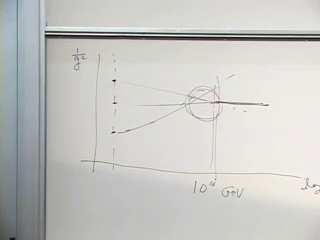
\includegraphics[width=0.74\textwidth]{lecture_10_figure_07.png}
\lectureframe{01:36:32.500}
\caption{逆ゲージ結合定数が\(10^{16}\,\mathrm{GeV}\)付近で互いに近づく様子の板書プロット。丸で囲まれた領域は、それらが不完全に交わる場所を示している。}
\label{fig:l10-running-board}
\end{figure}

大統一閾値より下では対称性は破れており、軽いスペクトルは完全な縮退した\(SU(5)\)多重項を満たさず、3つのベータ関数係数は異なっている。その結果、結合定数は異なる速率で走る。高いスケールでは、それらが共通の値に到達するかどうかが問われる：
\begin{equation}
\alpha_1(M_{\mathrm{GUT}})
\stackrel{?}{=}
\alpha_2(M_{\mathrm{GUT}})
\stackrel{?}{=}
\alpha_3(M_{\mathrm{GUT}}).
\label{eq:l10-unification-condition}
\end{equation}

非超対称な標準模型のスペクトルのみでは、線は\(10^{15}\)--\(10^{16}\,\mathrm{GeV}\)付近で互いに近づくが、かなりの量だけずれる。講義では、一致の程度はおよそ15パーセントと述べられている。重要な偶然の一致は、これが陽子の安定性によって要求されるスケールでもあるということである。

\section{最後の中性子に関する質問}

\begin{classroomqa}
\audiencequestion{陽子崩壊の図における spectator アップクォークがダウンクォークに置き換えられたなら、これは中性子崩壊を記述するだろうか、そして\(X\)ボソンは問題になるだろうか？\lecturetimestamp{01:36:40}}
\lecturerresponse{それは\(n\to e^++\pi^-\)のような大統一中性子チャネルを定義するだろうが、それは自由中性子のよく知られた崩壊ではない。通常の中性子ベータ崩壊は\(n\to p+e^-+\overline\nu_e\)であり、弱い相互作用を通じて進行する。もし陽子--中性子の質量順序が逆であれば、ベータ安定性もまた逆になるだろうが、はるかに遅い大統一チャネルは残り得る。}
\end{classroomqa}

この区別は、運動学と新しい相互作用を分ける。どの核子がベータ崩壊するかは陽子--中性子の質量差に依存し、\(X/Y\)交換によるバリオン数破れは、別の、途方もなく抑制された機構である。

\section{超対称性とより大きな視点}

超対称なパートナースペクトルを加えると、式~\eqref{eq:l10-running}のベータ関数係数が変化する。講義の説明では、3つの外挿された結合定数は約1パーセントの精度で一致する。これは超対称性や大統一を証明するものではないが、2つのアイデアがしばしば一緒に議論される経験的な理由である。

物質多重項はさらに統一することができる。\begin{equation}
SO(10)\supset SU(5),
\end{equation} のもとで、一つのスピノル表現は \begin{equation}
\mathbf{16}
\longrightarrow
\mathbf{10}\oplus\overline{\mathbf5}\oplus\mathbf1.
\label{eq:l10-so10}
\end{equation} と分解する。一重項は自然に左手系反ニュートリノ、あるいは同等に右手系ニュートリノの荷電共役と同一視される。したがって、拡張された世代の16個の場はすべて、一つの既約な \(SO(10)\) 多重項に収まる。

陽子崩壊実験は、事象が観測されないときに寿命の上限を引き上げることによって、このアイデアを検証し続けている。超対称大統一模型は単一の普遍的な陽子寿命を与えない：追加の重い場や超対称パートナーに依存する演算子が、支配的なチャネルと速率を広い範囲で変え得る。

\editorialnote{超対称大統一では、カラートリプレットヒッグスの交換が、ここで議論した6次元ゲージボソン演算子に加えて、5次元のバリオン数破れ演算子を生成し得る。それらの係数は重いスペクトル、フレーバー構造、超対称パートナー質量に強く依存し、このことが、超対称性だけから単一の寿命が導かれるわけではないという講義の警告を説明している。}

永続する教訓は、判決ではなく緊張関係である。群論はクォークとレプトンを驚くべき経済性で一緒に収め、走る結合定数は共通の高いスケールをほのめかし、超対称性は数値的なほのめかしを鋭くする。同じ構成はまた、クォークがレプトンへと危険に変換されることを予言する。したがって、成功するあらゆる版は、優雅さを保ちながら、陽子をほとんど想像を絶するほど長い間安定に保たなければならない。講義の締めくくりの精神で言えば、我々の陽子がすべて安定であり続けますように。
